\section{Results}
\label{sec:result}

\begin{table*}
\centering
\begin{tabular}{l|r|r|r|r|r}
Model
& Vertices
& Segments
& Segmentation time
& Partial matching time
& Correspondence clustering time\\
\hline
%%%RRM Use captial letter for all model names
Armadillo  & 172,974  & 9 &  1.6s   & 959.0s & 7.8s \\
Chetah     &   5,000  & 7 &  0.2s   & 588.2s & 5.2s  \\
Dinosaur   &  69,215  & 7 &  3.2s   & 522.7s & 5.1s   \\
Eager      &  14,618  & 6 &  0.5s   & 403.1s & 3.2s \\
Gargoyl    & 250,003  & 6 &  3.6s   & 448.9s & 3.9s  \\
\hline
\end{tabular}
\caption{Times taken by our algorithm, using a 1.6GHz Intel Core i7 CPU laptop with 4GB of RAM.
}
\label{tab:timing}
\end{table*}

Our algorithm has been tested on a variety of 3D shapes.
We visualize the discrete matches using similar colors to show symmetrically related parts.

We first show experimental results on clean, complete manifold meshes, without noise.
For such models, our algorithm provides a good initial segmentation for the partial matching, and we obtain  results which are in good agreement with those expected (e.g.\ Figures~\ref{fig:Eager} and~\ref{fig:Tiger}).

%%%RRM The objects are not exactly symmetric, so theere can be no "perfect" results.
%%%RRM Actually. I disagree. The head has a mirror symmetry which is not detected;
%%%RRM same for the animal's back
%%%RRM
%%%RRM Whether the legs should be recognised as copies or not depends on how approximate you let
%%%RRM the approximate symmetries be.
%%%RRM
%%%RRM For some applications it would be good to see all 4 legs as the same.
%%%RRM For other applications you would want to detect front and back legs as different.
%%%RRM The eagle figure does not make it clear what the detected symmetries are.

\begin{figure}[t]
\centering
  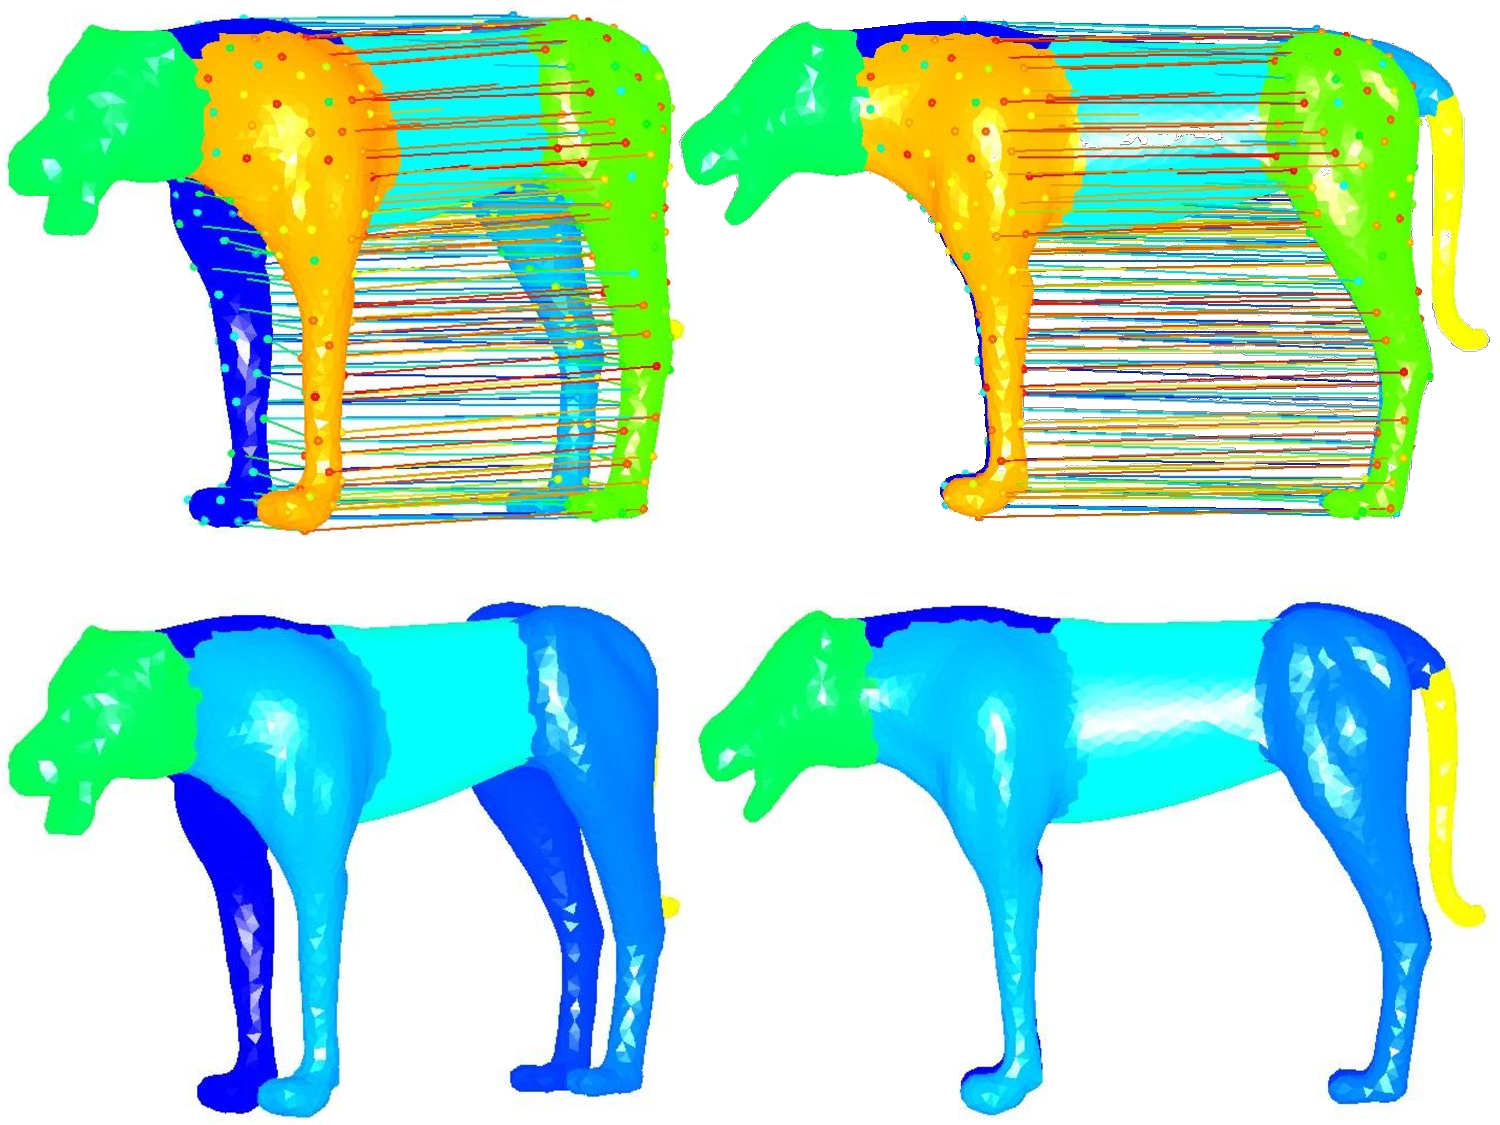
\includegraphics[width=0.99\linewidth]{figures/chetah.pdf}
  \caption{The four legs of the cheetah are detected as symmetric copies when using configuration $c=0.2/n$ and $m=100 \times n$, where $n$ is the user-defined segmentation number.
  %%%RRM what is n?
}
\label{fig:Tiger}
\end{figure}

As our algorithm depends on segmentation, uniform sampling of partial matching,
and transformation space clustering, the matching results do not depend on the representation or exact sampling (e.g.\ mesh) used.
Figure~\ref{fig:Point} demonstrates that our algorithm can be applied to shapes in  point set form.
Simultaneously, it also demonstrates that our algorithm is insensitive to  mesh variations, as the left and right sides of the dinosaur were sampled with quite different spatial resolutions.

\begin{figure}[t]
\centering
  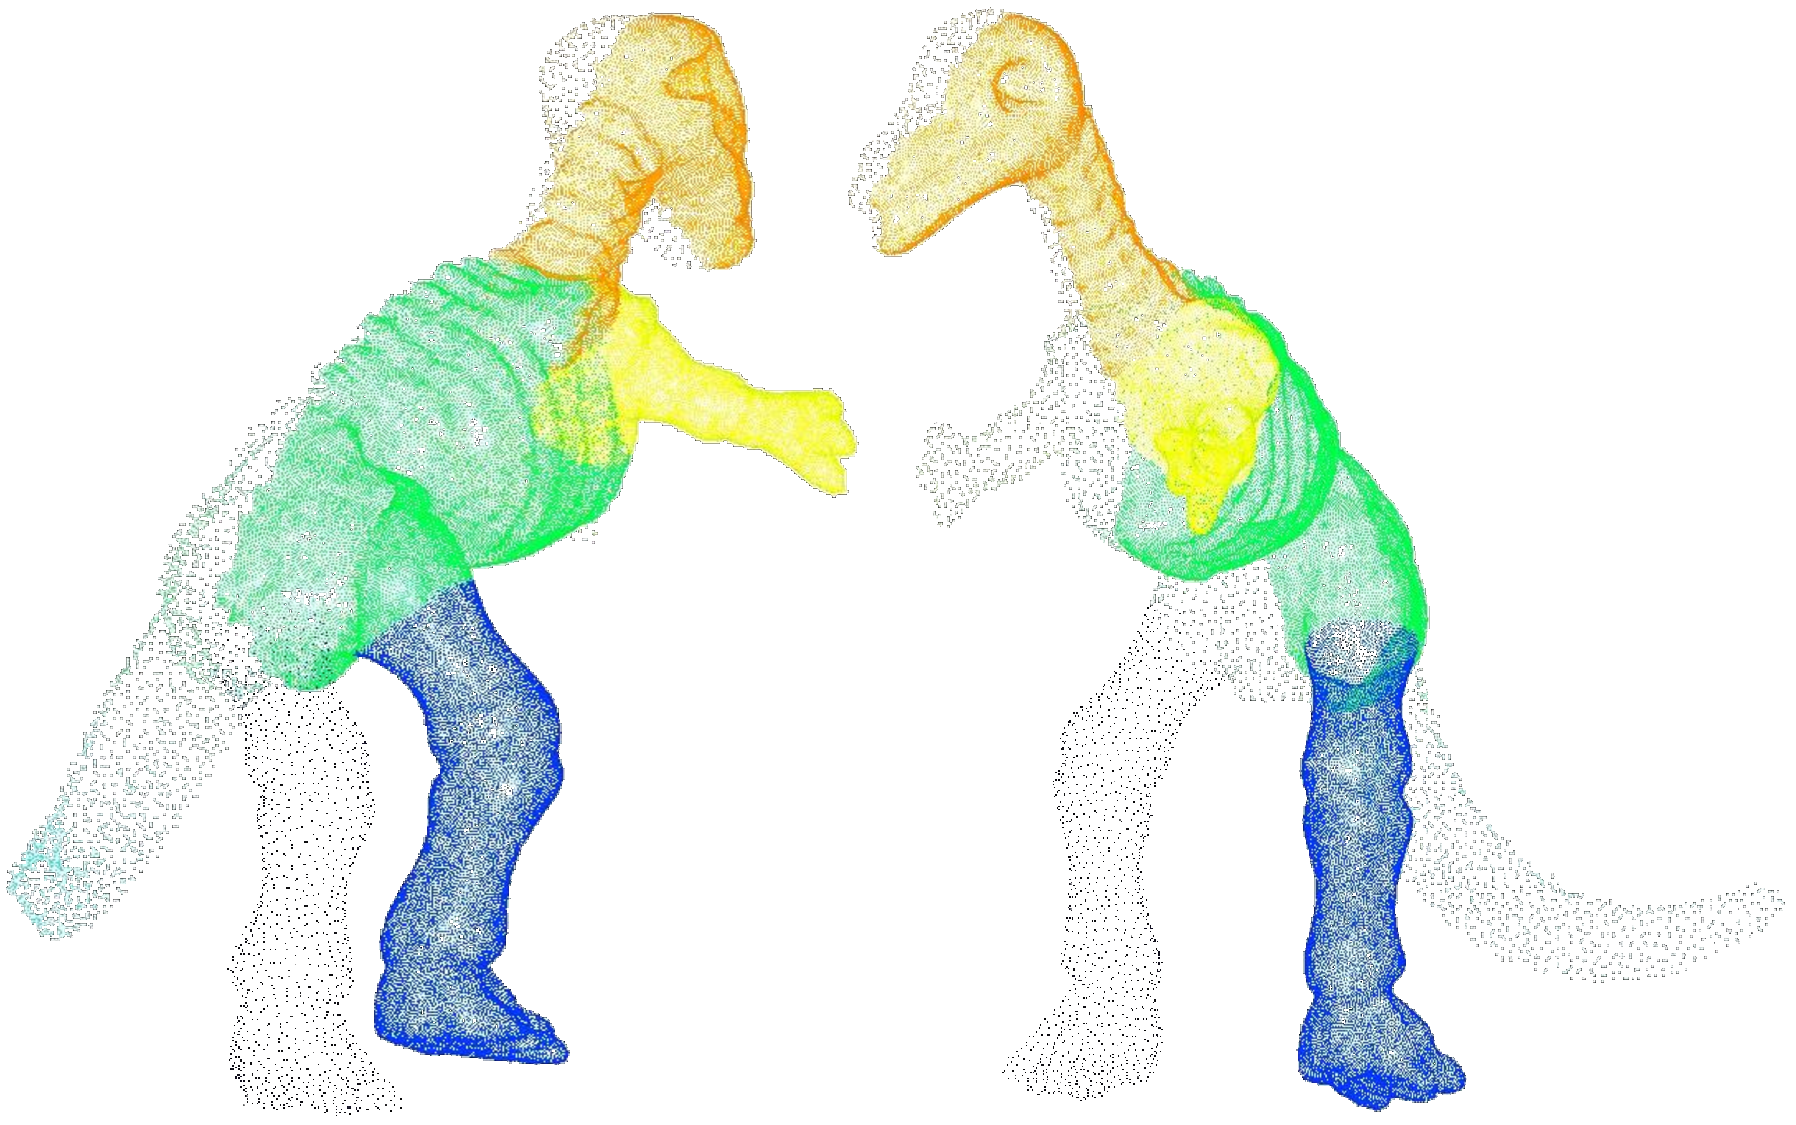
\includegraphics[width=0.99\linewidth]{figures/dinosaur.pdf}
  \caption{Symmetry detection in a dinosaur model represented as a point set with  different spatial resolutions on  left and right.}
\label{fig:Point}
\end{figure}

Figure~\ref{fig:Gargoyl} shows an example containing three different symmetry groups composed of reflection, rotation, and translation.
The symmetries are detected in coarse-to-fine steps based on  hierarchical segmentation.
At the coarse level, all major reflection symmetries are faithfully recovered,
while at the fine level, many rotational and translational symmetries are also detected.
Note that~\cite{berner2011} cites this example as on on which its state of the art algorithm  does
not perform well.

Results of processing complete and incomplete armadillo models are shown in Figure~\ref{fig:Arm},
demonstrating our ability to handle incomplete shapes.
In both cases, the algorithm computes a global reflection plane based on all final correspondences; the plane is almost identical in  both cases.

\begin{figure}[t]
\centering
  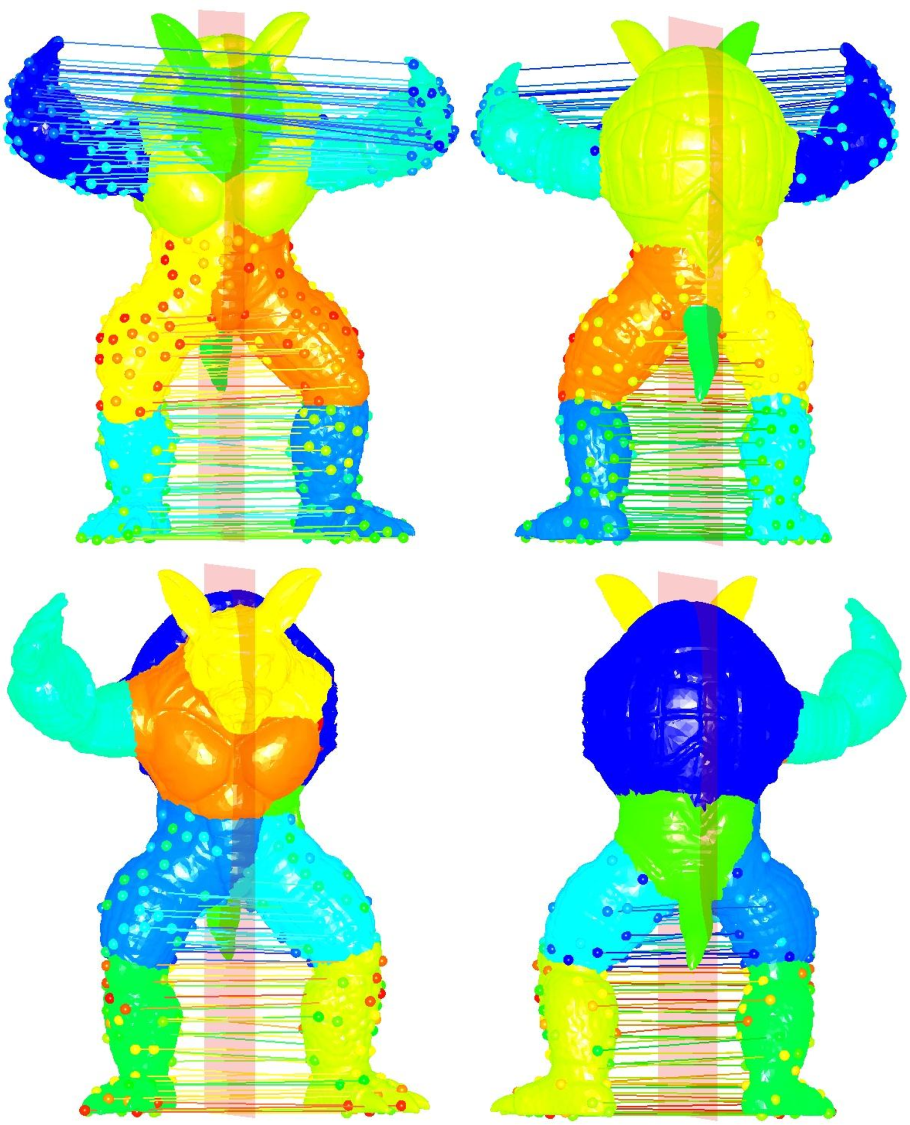
\includegraphics[width=0.99\linewidth]{figures/Armadillo.pdf}
  \caption{The global reflection plane is almost identical, for both complete and incomplete armadillo models (note the missing arm).}
\label{fig:Arm}
\end{figure}

Finally, we demonstrate iterative use of segmentation and symmetry detection steps to improve the output,  both in terms of shape segmentation and symmetry detection.
Initially, the segmentation of the shape
%%%RRM what shape?
is merely `satisfactory', as the shape is complex.
Following segmentation,  symmetry is detected as before. Using the detected reflection symmetry information, we further improve the segmentation.
%%%RRM How? This needs to go in the method description section of the paper, not in the results!
Figure~\ref{fig:Gargoyl} shows the initial segmentation and symmetry detection, and the refined results after two iterations.

%\begin{figure}[t]
%\centering
%  %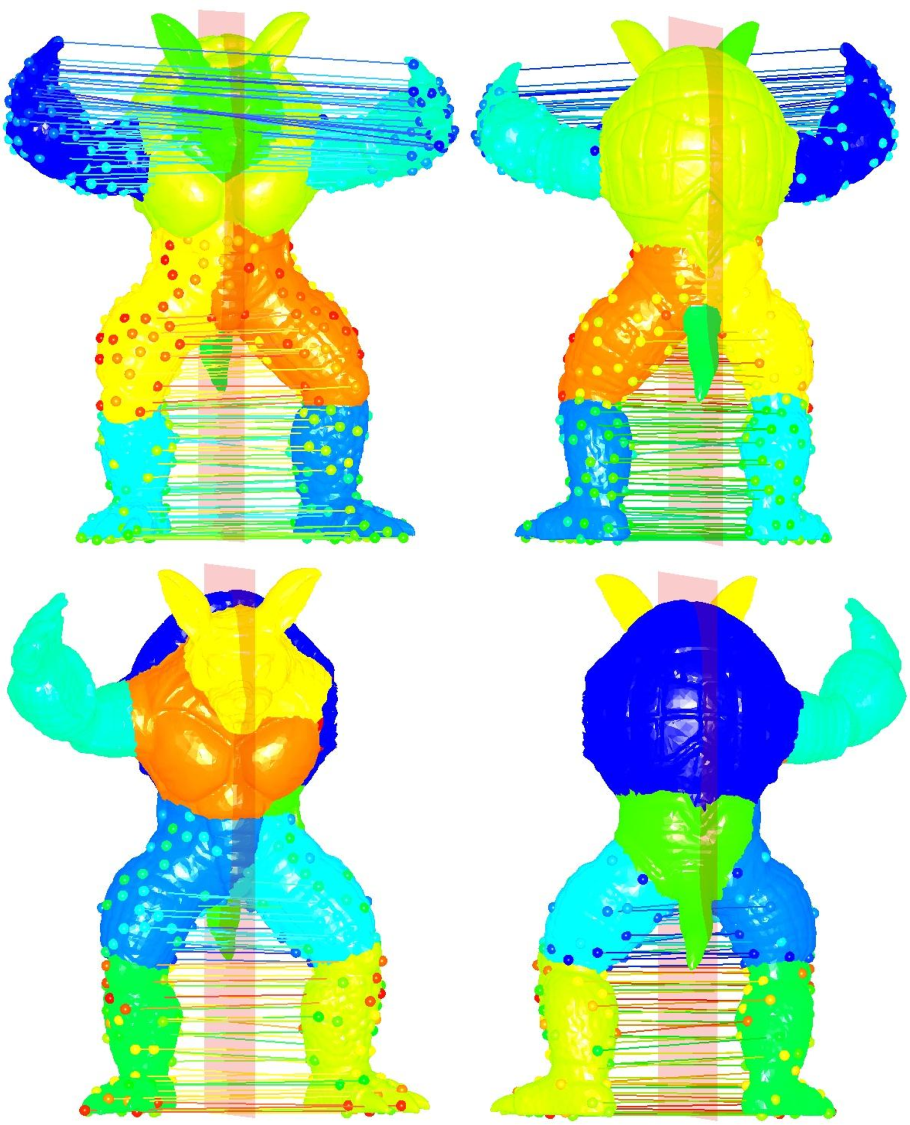
\includegraphics[width=0.99\linewidth]{figures/Armadillo.pdf}
%  \caption{The iterative segmentation and symmetry detection. Top: the initial results, below: the results after two iteration.}
%\label{fig:iteration}
%\end{figure}

The performance data in Table~\ref{tab:timing} shows computation times for various 3D shapes.
Partial matching takes more time than segmentation, but is less sensitive to the number of vertices in each shape: sampling is linearly dependent on the number of segmented parts.

